\section{Overview}

For hybrid virtual environments in clouds, RDMA virtualization not only needs to be unified, but also maintains high performance and manageability. Therefore, our design goals are as follows:

\begin{itemize}
	\item {\verb|Unification|}: Only single RDMA virtualization framework needs to be deployed in hybrid virtual environments and it provides centralized management.
	To form unified RDMA virtualization, single centralized virtual layer should be set up, which is provided to virtual machines and containers with general interfaces.
	\item {\verb|High performance|}: Performance of virtual RDMA should be close to native RDMA in terms of throughput, latency, or CPU load. Meanwhile it should suit for large-scale virtual cluster.
	\item {\verb|High manageablility|}: Basic managment shoud be meet for the clouds, such as, performance isolation, virtual network management or  portability.
\end{itemize}

% 简单介绍uniRDMA框架的工作过程
To achieve above goals, we propose a software RDMA virtualization framework, namely uniRDMA. As Figure~\ref{fig:framework-overview} shows, uniRDMA consists of vRNICs(including its' driver/library in VMs or containers) and the virtual layer:

vRNICs is a simple software emulation of physical RNIC. Each vRNIC is instanced in the virtual layer when VM or container's RDMA applications start. The RDMA commands of applications can be transported to vRNIC through guest driver or container libraries. Besides, RDMA resources (e.g. QPs and DoorBells) in vRNICs are mapped to physical RNIC and upper applications. Thus, the data commands in application can be executed locally for high-performance.

The virtual layer is also in host user-space. We design it for centralized management of vRNICs. It controls all RDMA devices through RDMA verbs library in host user space. Meanwhile, vRNICs are configured in the virtual layer to construct virtual RDMA network, e.g. vRNIC addresses and routing rules.

\begin{figure}[!ht]
	\centering
	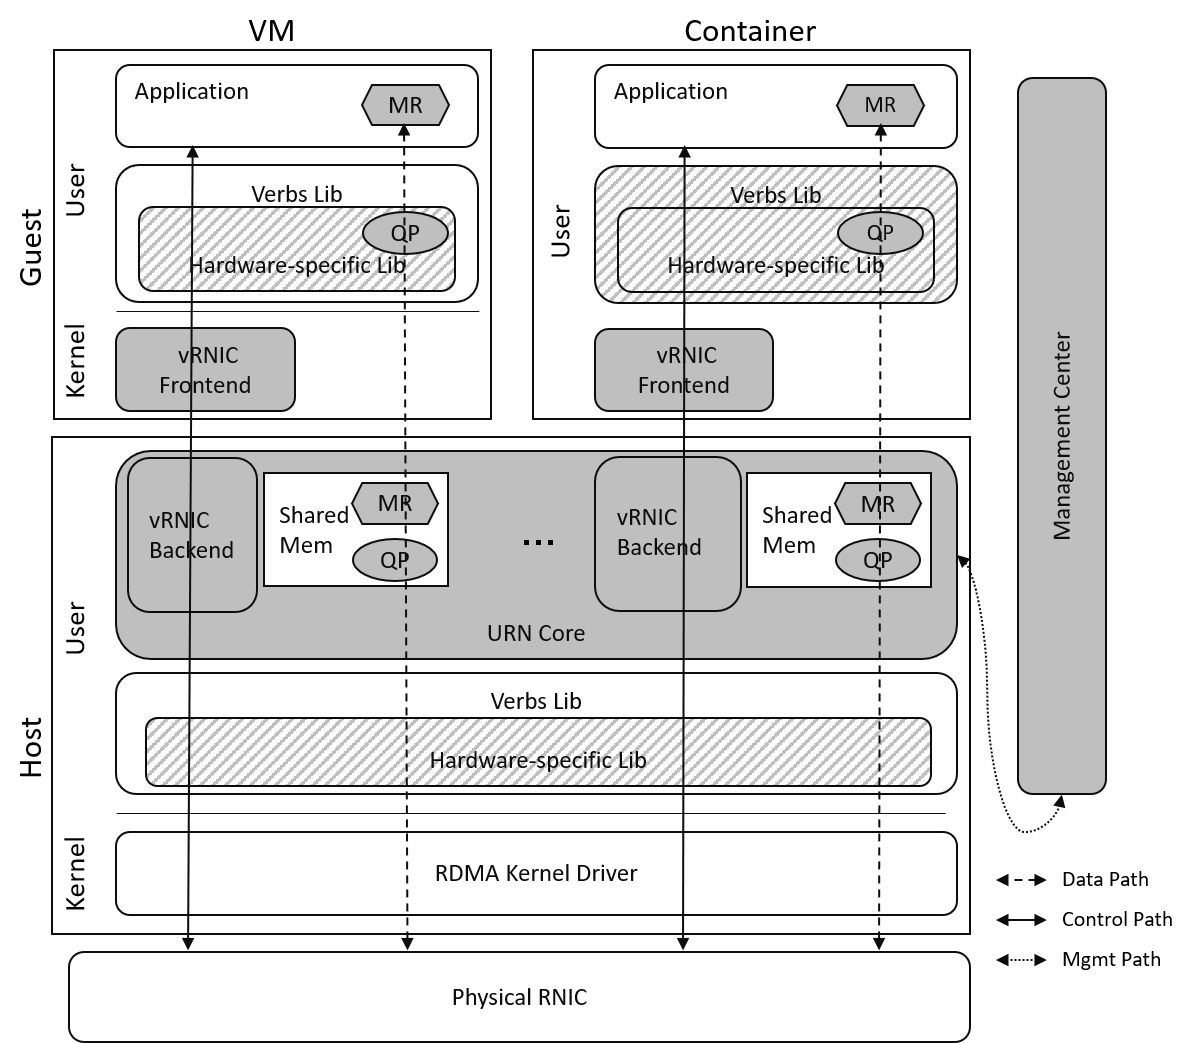
\includegraphics[width=0.9\linewidth]{images/framework-overview.png}
	\caption{uniRDMA Framework Overview}
	\label{fig:framework-overview}
\end{figure}
